\documentclass{article}
\usepackage[T1]{fontenc}
\usepackage{graphicx}
\usepackage{amsthm}
\usepackage{amsmath}
\usepackage{xcolor}
\usepackage{footnote}
\usepackage{hyperref}
\hypersetup{colorlinks=True,
            linkcolor=brown}
\usepackage{subcaption}
\usepackage{caption}
\usepackage{amssymb}

\begin{document}

\title{Notes on SSA}
\author{Jonsa Pichat}
\date{18 November 2019}
\maketitle


\section{SSA}
\label{ssa}

Singular spectrum analysis (SSA) can be defined as principal component analysis (PCA) for univariate time series data. As a reminder, PCA consists of the decomposition of a covariance matrix $X^TX$, where $X\in\mathbb{R}^{n\times m}$ is a data matrix ($n$ being the number of samples, $m$ the number of features and the objective is dimension reduction). 

On the other hand, SSA consists of the spectral decomposition of a lag-covariance matrix, also $X^TX$, though $X$ (called the trajectory matrix) contains "the complete record of patterns that have occurred within a window of size $L$" (or embedding dimension). It is defined such that, given a centred time series $y=y_1, \dots, y_N$ (with $N=L+K-1$) of finite rank, one has:

  % \left(
\[X=
  \begin{bmatrix} 
    y_{1} & y_{2} & y_{3} & \dots  & y_{L} \\
    y_{2} & y_{3} & y_{4} & \dots  & y_{L+1} \\
    y_{3} & y_{4} & y_{5} & \dots  & y_{L+2} \\
    \vdots & \vdots & \vdots & \ddots & \vdots \\
    y_{K} & y_{K+1} & \dots & \dots  & y_{L+K}
\end{bmatrix}
\]


Elser and Tsonis state that "by using lagged copies of a single time series, [we] can define the coordinates of the phase space that will approximate the dynamics of the system from which the time record was sampled".\\

% The difference between the structures of the data matrix in PCA versus SSA is precisely what contributes to their different behaviors.

\subsection{Overview}


SSA consists of 2 stages:
\begin{enumerate}
  \item \textbf{decomposition}: (i) \textit{embedding} (see trajectory matrix, $X$ above) and (ii) \textit{decomposition}: SVD is applied to $X$ (equivalently, one may do an eigendecomposition of the covariance matrix) to obtain a decomposition into elementary rank-one matrix components.
  \item \textbf{reconstruction}: (iii) \textit{grouping}: grouped matrix components are created in a clever way and (iv) \textit{diagonal averaging}: those are back-transformed to provide a decomposition of the time series.
\end{enumerate}

% By discarding the projections that correspond to the unwanted sources (such as the noise or artifact sources), i.e. dimensionality reduction, and then inverting the transformation, we effectively perform a filtering of the signal.

\subsection{Decomposition}

The trajectory matrix is obtained via embedding, using {\fontfamily{pcr}\selectfont WindowTransform}, and it is decomposed using SVD: it provides the decomposition: $X=USV^T$, where the  columns of U and V are bases for the row and column spaces of $X$.

\begin{align}
X &= \sum_i\sigma_iU_iV_i^T\nonumber \\
  &= \sum_i \Pi_i X\nonumber
\end{align}

where (i) $U,V$ are left singular and right singular vectors of $X$, or where (ii) $\Pi_i=U_i U_i^T$ is a projection matrix (with $U_i$, the eigenvectors of $X^TX$)\footnote{since $V_i=\frac{1}{\sigma_i} X^TU_i$, one can rewrite the SVD decomposition of $X$ as $US(X^TUS^{-1})^T$}.\\


\begin{figure}
  \centering
  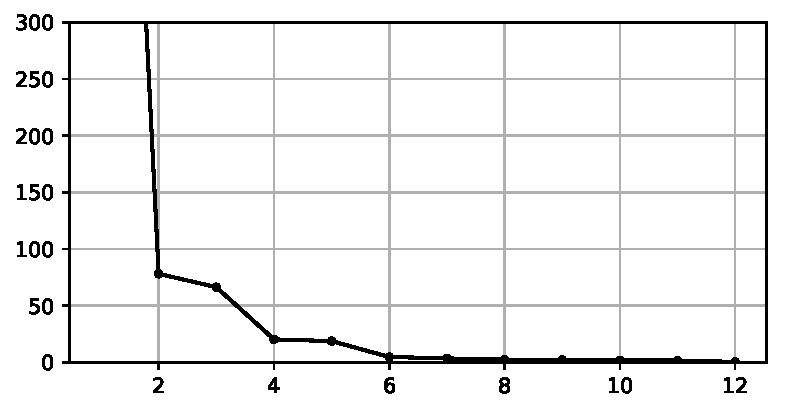
\includegraphics[scale=0.5]{figures/fig0}
  \caption{eigenvalues of lag-covariance matrix from passengers series. The first eigenvalue (related to the trend) is not shown here, because it is too large. In general, correlated components have similar eigenvalues (see (2,3) and (4,5), and noise can be related to small eigenvalues that decrease linearly (see ~6 to 12). Here, $k$=6 meaning that one should use at most $n_e$=6 leading eigenvectors, and components (2,3) and (4,5) should be grouped (so $n_c=3$).}
  \label{fig:f0}
\end{figure}


\begin{figure}
  \begin{subfigure}{0.5\textwidth}
    \centering
    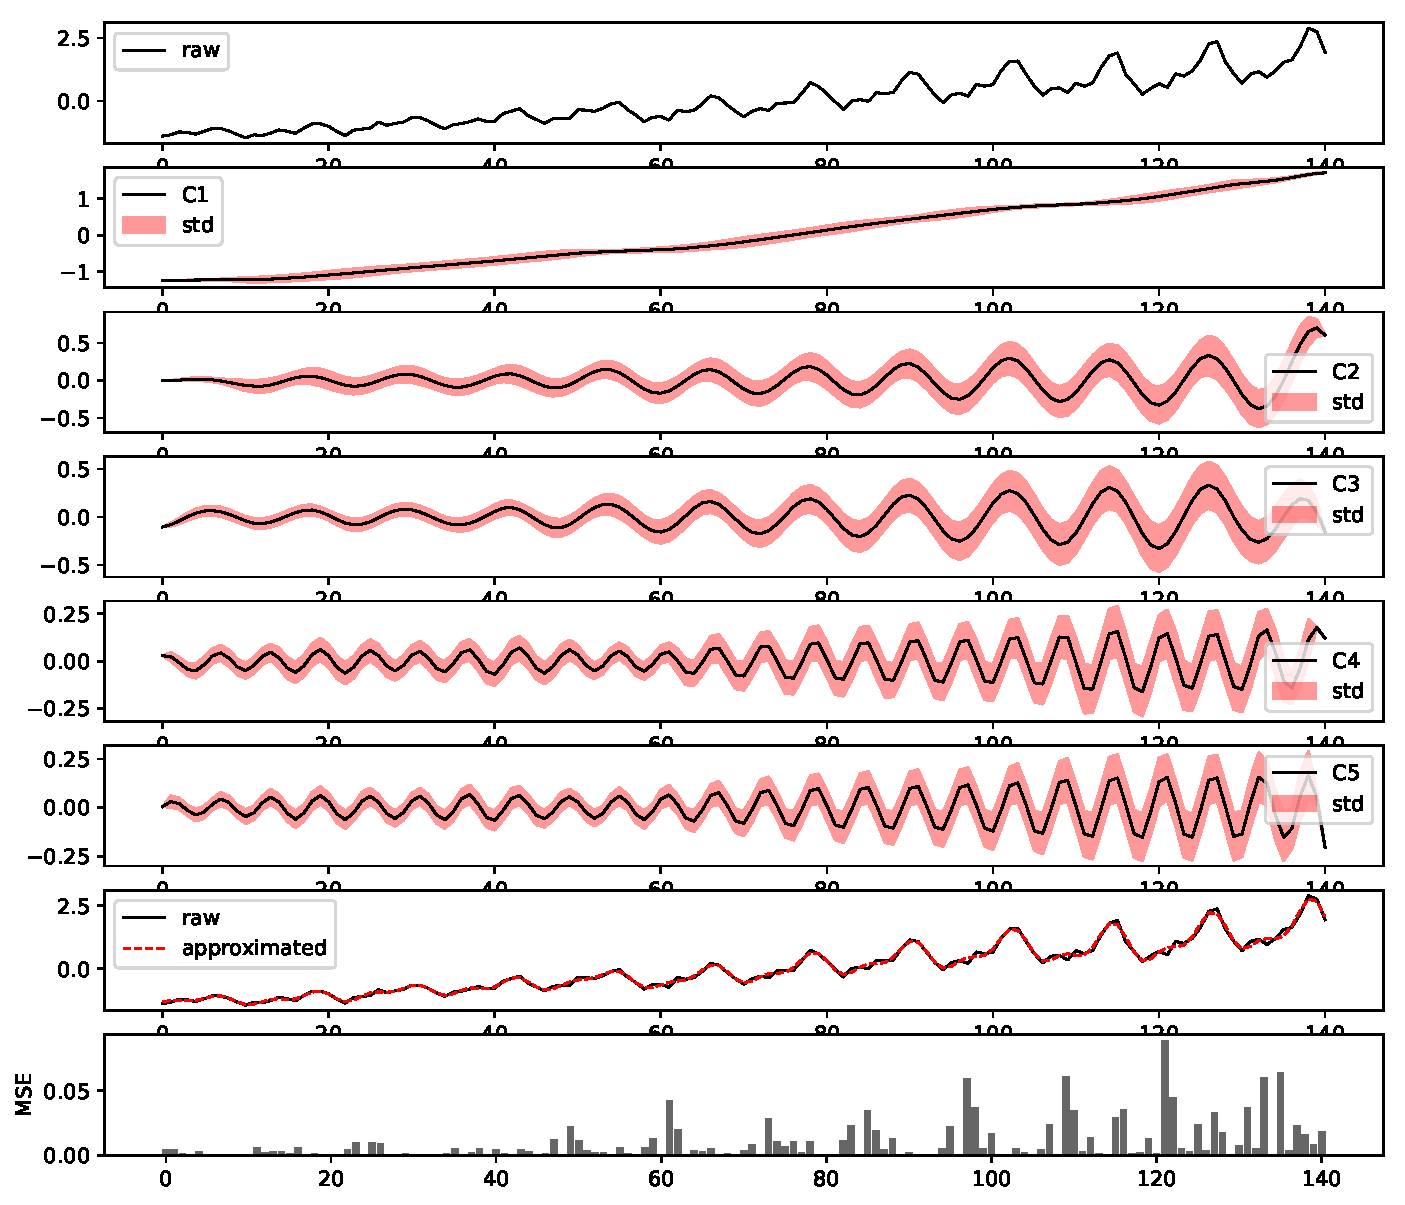
\includegraphics[scale=0.23]{figures/fig2a}
    \caption{}
    \label{fig:f2a}
  \end{subfigure}%
  \hspace{3mm}
  \begin{subfigure}{0.5\textwidth}
    \centering
    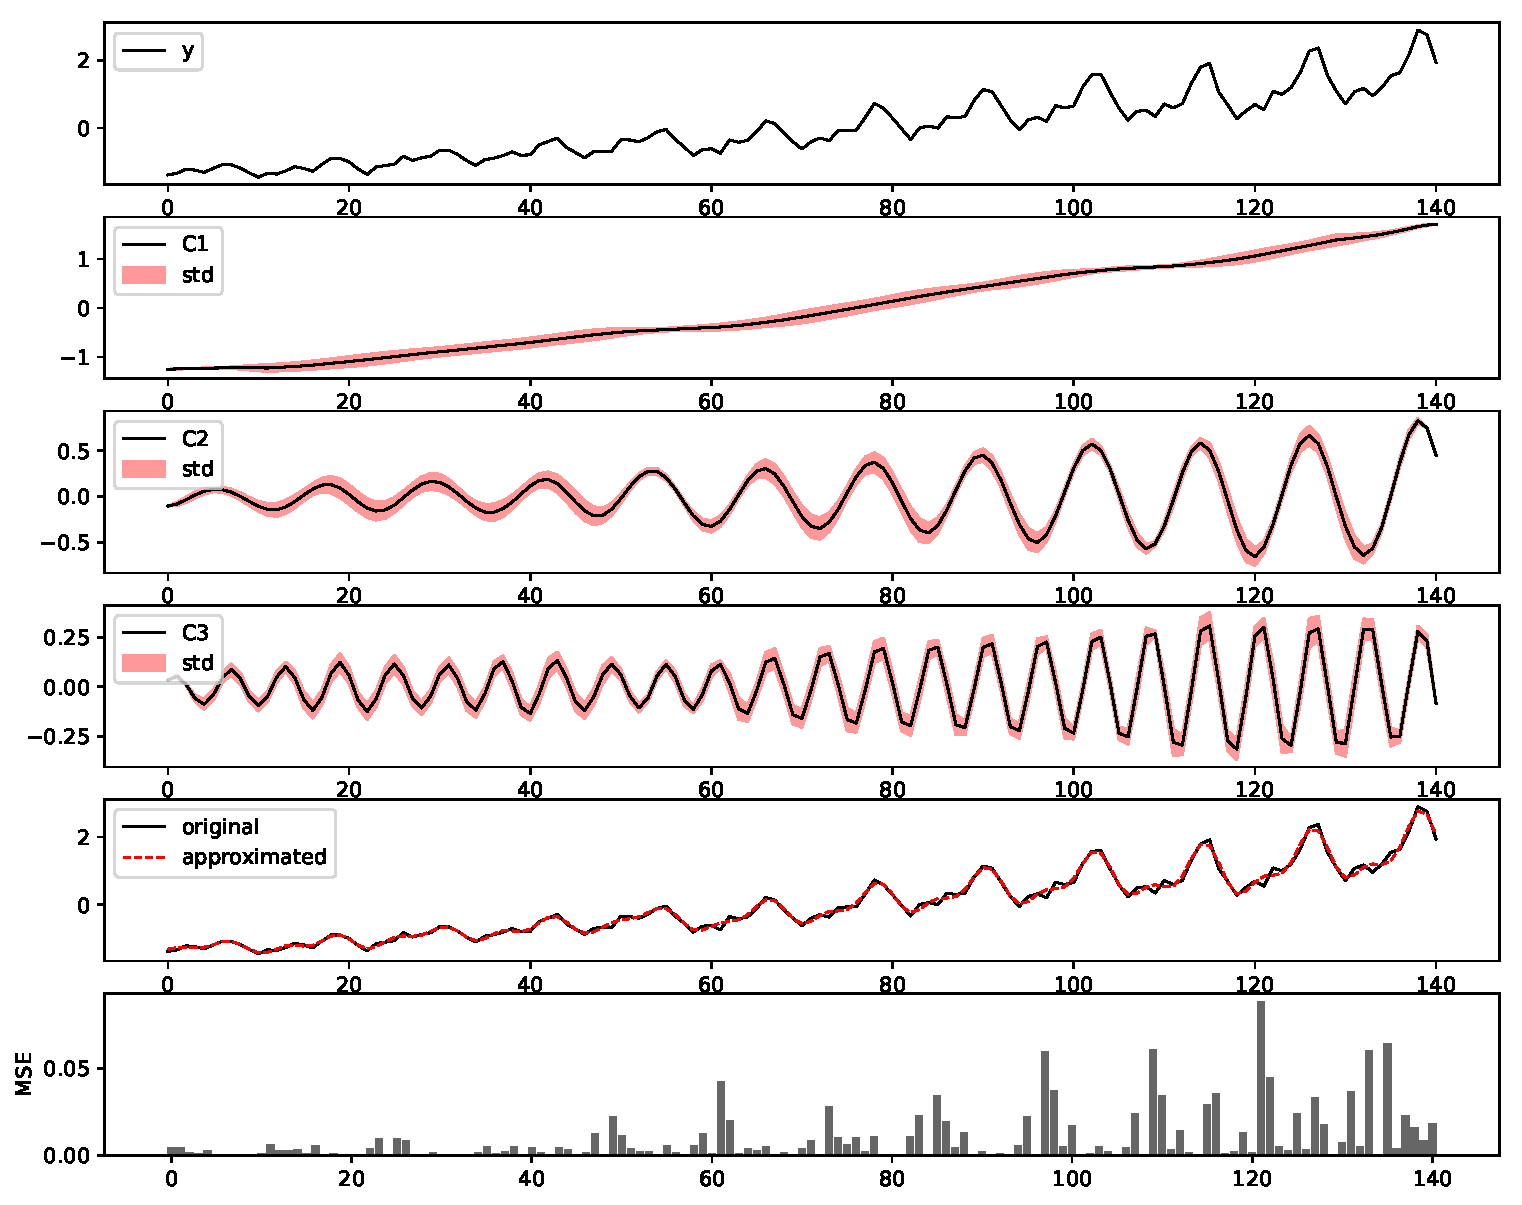
\includegraphics[scale=0.23]{figures/fig1a}
    \caption{}
    \label{fig:f1a}
  \end{subfigure}
  \vspace{4mm}

  \begin{subfigure}{0.5\textwidth}
    \centering
    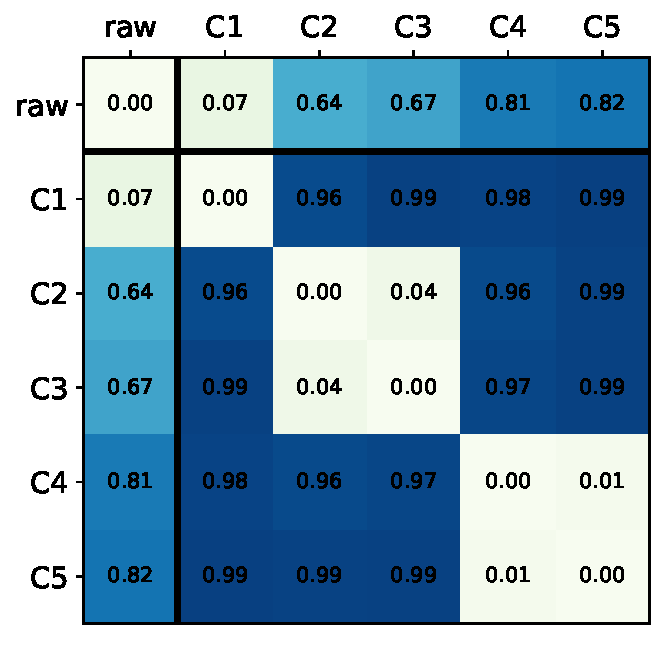
\includegraphics[scale=0.33]{figures/fig2b}
    \caption{}
    \label{fig:f2b}
  \end{subfigure}%
  \begin{subfigure}{.5\textwidth}
    \centering
    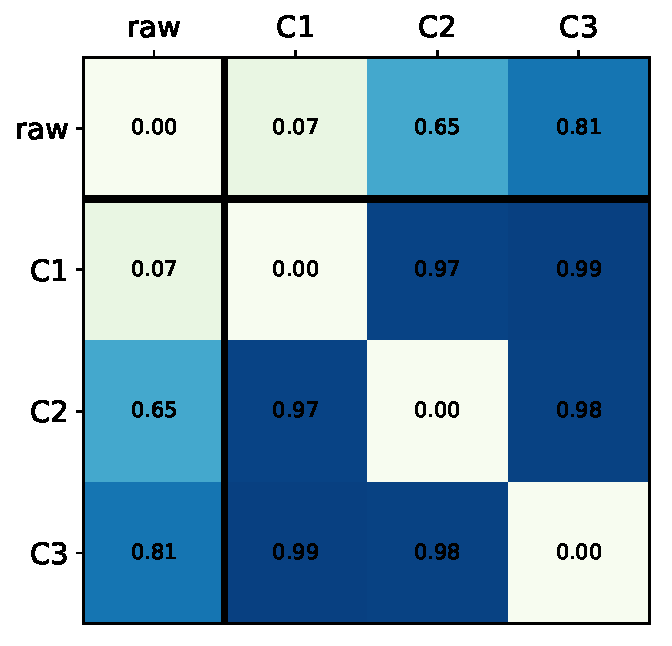
\includegraphics[scale=0.33]{figures/fig1b}
    \caption{}
    \label{fig:f1b}
  \end{subfigure}  

  \caption{SSA decomposition without (\ref{fig:f2a}) and with (\ref{fig:f1a}) grouping (using weighted-correlations) of passengers series into respectively $n_c$=5 and $n_c$=3 ($n_e$=5); recall that grouping is "turned off" when $n_c=n_e$. The red shaded regions in the components plots correspond to standard deviations of antidiagonals during \textit{diagonal averaging} (reconstruction). Resulting pairwise dependence is shown in the distance matrix (the larger, the more uncorrelated) (\ref{fig:f2b} and \ref{fig:f1b}). Note that, (C1, C2) and (C3, C4) are clearly correlated; this is confirmed by Fig.~\ref{fig:f0} and those were (automatically) grouped to give the decomposition shown in \ref{fig:f1a}.}
  \label{fig:f1}
\end{figure}



One thereby has the approximation of $X=\sum_{i=1}^r X_i$, as a truncated sum of rank 1 quasi-Hankel matrices. This is the best approximation in terms of Euclidean distance\footnote{the problem of low-rank approximation of a data matrix $D$ is defined as the minimisation of the Frobenius norm $||D-\widetilde{D}||_F$ $\Big($def: $||A||^2_F=\textmd{Trace}(A^TA)=\sum \sigma^2_A\Big)$ over $\widetilde{D}$ subject to $\textmd{rank}(\widetilde{D})<r$, the desired rank. It has an analytic solution in terms of the SVD of $D$.}, to any rectangular matrix. Note that by discarding the projections that correspond to the unwanted sources---such as the noise or artifact sources, usually associated with lower eigenvalues (Fig.~\ref{fig:f0})---and then inverting the transformation, we effectively perform a filtering of the signal (Fig.~\ref{fig:f1}). \\


The way it is implemented, one can either:
\begin{itemize}
  \item choose only a number of components, $n_c$ ({\fontfamily{pcr}\selectfont n\_components}), in which case, the number of leading eigenvectors used for matrix approximation is the smallest $k$ such that $\sum_{i=1}^{k}\lambda_i / \sum_{i}\lambda_i>t$, where $t$ is a variance threshold arbitrarily set to 99\%, and $\lambda_1>\lambda_2,\dots$ are the eigenvalues of the lag-covariance matrix. Note that Donoho\footnote{(Gavish and Donoho, 2014) The Optimal Hard Threshold for Singular Values is $4/\sqrt{3}$ (\href{https://www.arxiv.org/abs/1305.5870}{arXiv:1305.5870})} proposed other thresholds (on $\sqrt{\lambda_i}$)---that depend on matrix dimensions and whether the noise level is known---which could be used in addition/replacement. From there, if $n_c>k$, the decomposition is elementary and one is likely to obtain noisy components (associated with small eigenvalues); otherwise, $k$ elementary components will be grouped into $n_c$ components.
  \item choose both a number of components, $n_c$ and a number of eigenvectors ({\fontfamily{pcr}\selectfont n\_leading\_ev}), $n_e$ with $n_c<n_e$. If $n_e>k$, then $n_e$ first eigenvectors are used for elementary projections, but one must know that those associated with small eigenvalues are likely to be noise; the opposite case might result in a coarse decomposition (and therefore a rough approximation) as the proportion of variance explained is less that 99\% (here). The elementary components are then grouped into $n_c$ components, according to a grouping method.
\end{itemize}



\begin{figure}
  \centering
  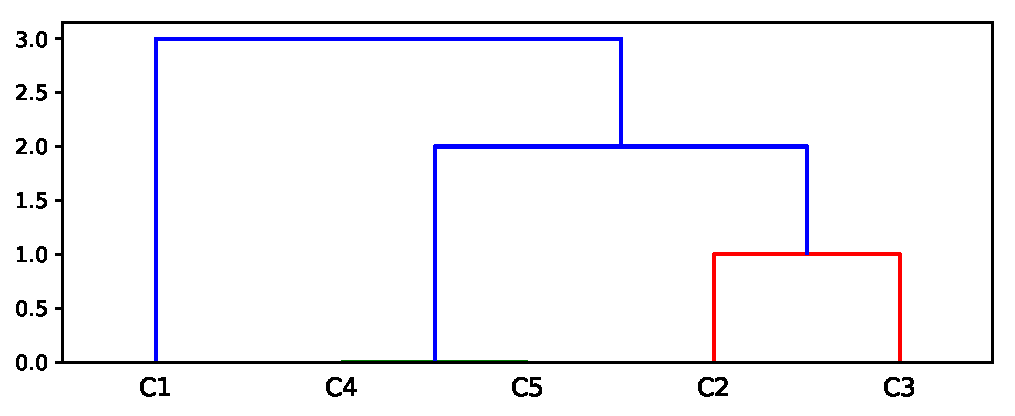
\includegraphics[scale=0.4]{figures/fig3}
  \caption{Hierarchical clustering (complete linkage) of elementary components C1, ..., C5 that come from the decomposition of passengers series ($n_c=n_e$=5). One can see that requesting $n_c$=3 gives \{C1 (trend), (C2+C3), (C4+C5)\}. Note that, should one ask for $n_c$=4, grouping would provide the set \{C1, C2, C3, (C4+C5)\}, which agrees with the distance matrix from Fig.~\ref{fig:f2b}: $d(\textmd{C4}, \textmd{C5})<d(\textmd{C2}, \textmd{C3})$; and similarly, $n_c$=2 would give \{C2, (C2+C3+C4+C5)\}.}
  \label{fig:f2}
\end{figure}



\subsection{Grouping}
Since some of the elementary components may end up being correlated, we group them using hierarchical clustering (Fig~\ref{fig:f2}). The distance matrix, $D$ can either be $D_{ij}=1-\rho_{ij}$ where $\rho$ is called the weighted-correlation or w-correlation:

\begin{equation}
\rho_{ij} = \frac{<C^{(i)}, C^{(j)}>_w}{||C^{(i)}||_w ||C^{(j)}||_w} 
\end{equation}

where $C^{(i)}=\{c^{(i)}_m\}_{m=1,..,N}$ are the reconstructed elementary components $X_i$ (referred to as C1, C2, etc. in the plots) via diagonal averaging (see Section~\ref{da}); $<C^{(i)}, C^{(j)}>_w=\sum_m w_m c^{(i)}_m c^{(j)}_m$, with weights $w_m=\min(m, L, N-m)$ (i.e., the number of elements along the $m$-th antidiagonal of $X_i$ or $X_j$, since they have the same dimensions); $||C^{(i)}||_w=\sqrt{<C^{(i)}, C^{(j)}>_w}$. Weighted-correlation quantifies how well different components can be separated from each other and can be seen as a measure of orthogonality (it relies on a dot product): the more orthogonal, the closer to 0 (and $d_{ij}\rightarrow 1$).

Else, the distance matrix can simply be the Euclidean distance between eigenvalues, though we observed more stable and interpretable results using the former.


\subsection{Diagonal averaging}
\label{da}
As the name suggests (actually it does not, strictly speaking), diagonal averaging consists of averaging elements of the antidiagonals of $X_i$. Because elementary components are only quasi-Hankel matrices, their antidiagonals are not constant, as opposed to the trajectory matrix defined in Section~\ref{ssa}. Averaging is one way to reconstruct time components, although it is not clear why it should be preferred to e.g. median, min or max. From there we can also extract the standard deviation; it is worth mentioning that grouped components are closer to Hankel matrices, as illustrated in Fig.~\ref{fig:f1} (grouping actually converges to a Hankel structure, since one gets closer to the original series as components are summed).

\subsection{Future work}
\subsubsection{"Reduced dimension" parameter}
The fix would consist of using (i) the threshold introduced in (Gavish and Donoho, 2014) (on which the user has no control), which sets an upper bound on the number of eigenvectors to use (ii) and a threshold on the explained variance. The former would be overridden by the latter (if given by the user) and likely result in coarser decompositions.


\subsubsection{Non-linear ssa}
The idea would be to use principal geodesic analysis (PGA) in order to consider the geometric structure of the lag-covariance matrix (which is disregarded in the Euclidean formulation of SSA). One could also think of carrying out grouping in Riemannian geometry using components' covariance matrices---as opposed to, for now, grouping them in the time domain (which requires their reconstruction) based on a correlation criterion. 

\section{Missing value imputation}
\subsection{Principle}
\subsection{Results}
\subsection{Future work}


\end{document}
